\documentclass[tikz,border=8pt]{standalone}
% Shared look for every TikZ diagram. Load with \input{../../tools/tikz-style.tex}
\usepackage[T1]{fontenc}
\usepackage{lmodern}
\renewcommand{\sfdefault}{lmr}  % diagrams use the same serif as the text
\usetikzlibrary{arrows.meta, positioning, shapes.geometric, calc, fit, backgrounds}
\definecolor{cblue}{HTML}{4C78A8}
\definecolor{corange}{HTML}{F58518}
\definecolor{cgreen}{HTML}{54A24B}
\definecolor{cred}{HTML}{E45756}
\definecolor{cpurple}{HTML}{B279A2}
\definecolor{cgrey}{HTML}{6B6B6B}
\tikzset{
  every picture/.style={font=\sffamily, line width=1.2pt},
  box/.style={draw=#1, fill=#1!12, rounded corners=4pt, align=center, inner sep=7pt, minimum height=1.1cm},
  box/.default=cgrey,
  arrow/.style={-{Stealth[length=3mm]}, draw=cgrey, line width=1.4pt},
  title/.style={font=\sffamily\bfseries\Large},
  note/.style={font=\sffamily\small, text=cgrey, align=center},
}
\AtBeginDocument{\hyphenpenalty=10000 \exhyphenpenalty=10000}

% #1 xshift, #2 title, #3-#6 matrix columns, #7 eigen-lines drawing, #8 caption
\newcommand{\panel}[8]{
  \begin{scope}[xshift=#1cm]
    \begin{scope}
      \clip (-3,-3) rectangle (3,3);
      \draw[cgrey!25, line width=0.4pt] (-3,-3) grid (3,3);
      \begin{scope}[cm={#3,#4,#5,#6,(0,0)}]
        \draw[cblue!45, line width=0.7pt] (-6,-6) grid (6,6);
      \end{scope}
      \draw[cgrey, line width=0.8pt] (-3,0) -- (3,0) (0,-3) -- (0,3);
      #7
    \end{scope}
    \node[font=\bfseries, align=center] at (0,4.1) {#2};
    \node[align=center, font=\small] at (0,-3.9) {#8};
  \end{scope}
}
\begin{document}
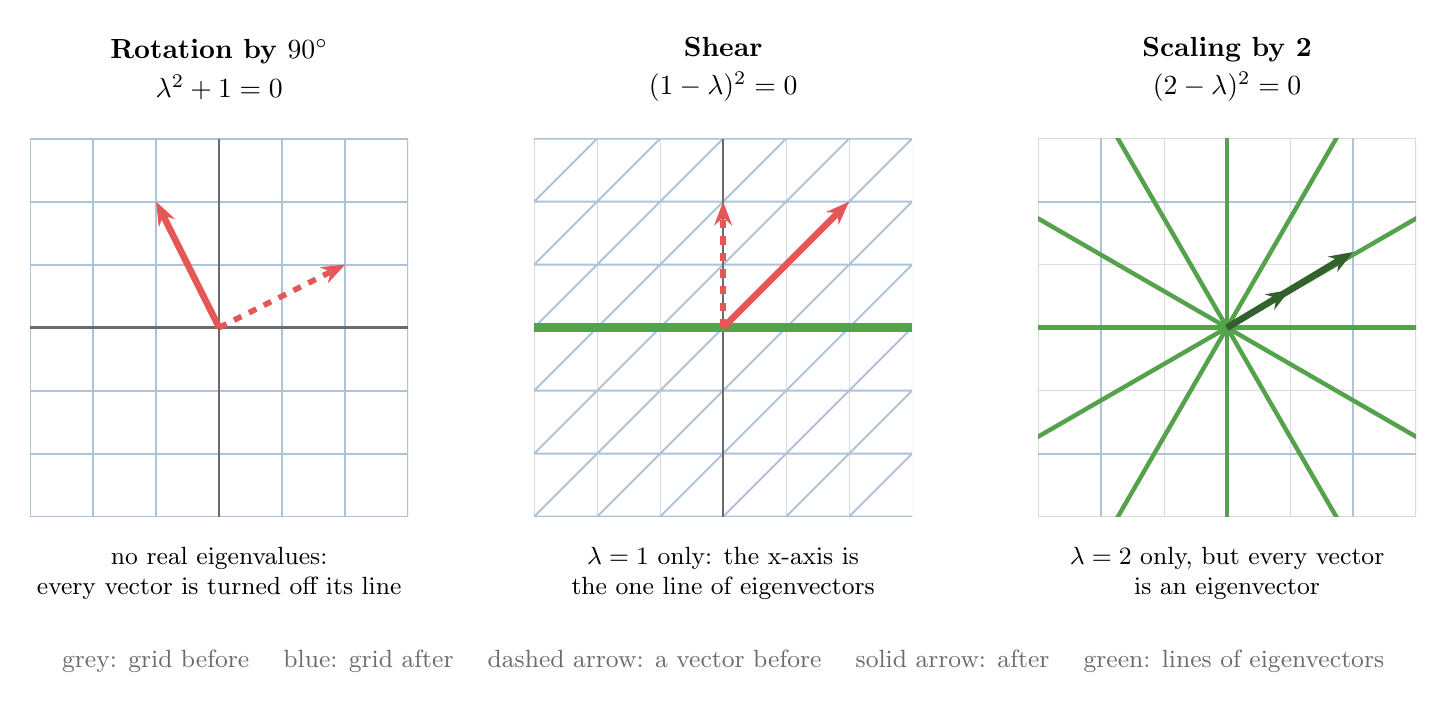
\begin{tikzpicture}[scale=0.8]
  \panel{0}{Rotation by $90^\circ$\\[2pt] $\lambda^2 + 1 = 0$}{0}{1}{-1}{0}
    {\draw[-{Stealth[length=3mm]}, cred, line width=2pt, dashed] (0,0) -- (2,1);
     \draw[-{Stealth[length=3mm]}, cred, line width=2.4pt] (0,0) -- (-1,2);}
    {no real eigenvalues:\\ every vector is turned off its line}
  \panel{8}{Shear\\[2pt] $(1 - \lambda)^2 = 0$}{1}{0}{1}{1}
    {\draw[cgreen, line width=3pt] (-3,0) -- (3,0);
     \draw[-{Stealth[length=3mm]}, cred, line width=2pt, dashed] (0,0) -- (0,2);
     \draw[-{Stealth[length=3mm]}, cred, line width=2.4pt] (0,0) -- (2,2);}
    {$\lambda = 1$ only: the x-axis is\\ the one line of eigenvectors}
  \panel{16}{Scaling by 2\\[2pt] $(2 - \lambda)^2 = 0$}{2}{0}{0}{2}
    {\foreach \a in {0,30,...,150} \draw[cgreen, line width=1.6pt] (\a:-4.5) -- (\a:4.5);
     \draw[-{Stealth[length=3mm]}, cgreen!60!black, line width=2pt, dashed] (0,0) -- (1,0.6);
     \draw[-{Stealth[length=3mm]}, cgreen!60!black, line width=2.4pt] (0,0) -- (2,1.2);}
    {$\lambda = 2$ only, but every vector\\ is an eigenvector}
  \node[note] at (8,-5.3) {grey: grid before \quad blue: grid after \quad dashed arrow: a vector before \quad solid arrow: after \quad green: lines of eigenvectors};
\end{tikzpicture}
\end{document}
